\documentclass[14pt]{extbook}
\usepackage{multicol, enumerate, enumitem, hyperref, color, soul, setspace, parskip, fancyhdr} %General Packages
\usepackage{amssymb, amsthm, amsmath, bbm, latexsym, units, mathtools} %Math Packages
\everymath{\displaystyle} %All math in Display Style
% Packages with additional options
\usepackage[headsep=0.5cm,headheight=12pt, left=1 in,right= 1 in,top= 1 in,bottom= 1 in]{geometry}
\usepackage[usenames,dvipsnames]{xcolor}
\usepackage{dashrule}  % Package to use the command below to create lines between items
\newcommand{\litem}[1]{\item#1\hspace*{-1cm}\rule{\textwidth}{0.4pt}}
\pagestyle{fancy}
\lhead{Progress Quiz 2}
\chead{}
\rhead{Version C}
\lfoot{7862-5421}
\cfoot{}
\rfoot{Spring 2021}
\begin{document}

\begin{enumerate}
\litem{
Solve the equation below. Then, choose the interval that contains the solution.\[ -13(-17x + 10) = -6(9x -3) \]\begin{enumerate}[label=\Alph*.]
\item \( x \in [0.34, 0.49] \)
\item \( x \in [0.55, 0.79] \)
\item \( x \in [-0.51, -0.39] \)
\item \( x \in [0.47, 0.67] \)
\item \( \text{There are no real solutions.} \)

\end{enumerate} }
\litem{
Find the equation of the line described below. Write the linear equation as $ y=mx+b $ and choose the intervals that contain $m$ and $b$.\[ \text{Parallel to } 8 x - 7 y = 11 \text{ and passing through the point } (-6, -3). \]\begin{enumerate}[label=\Alph*.]
\item \( m \in [0.96, 1.16] \hspace*{3mm} b \in [2.1, 3.7] \)
\item \( m \in [0.96, 1.16] \hspace*{3mm} b \in [3.8, 5] \)
\item \( m \in [-1.44, -0.93] \hspace*{3mm} b \in [-11.7, -7.1] \)
\item \( m \in [0.7, 1.12] \hspace*{3mm} b \in [3.8, 5] \)
\item \( m \in [0.96, 1.16] \hspace*{3mm} b \in [-4.1, -1.9] \)

\end{enumerate} }
\litem{
Find the equation of the line described below. Write the linear equation as $ y=mx+b $ and choose the intervals that contain $m$ and $b$.\[ \text{Perpendicular to } 7 x - 9 y = 5 \text{ and passing through the point } (-10, 9). \]\begin{enumerate}[label=\Alph*.]
\item \( m \in [-0.92, -0.67] \hspace*{3mm} b \in [-5.7, -2.3] \)
\item \( m \in [-2.25, -0.87] \hspace*{3mm} b \in [-5.7, -2.3] \)
\item \( m \in [-2.25, -0.87] \hspace*{3mm} b \in [17.7, 19.4] \)
\item \( m \in [1.18, 2.38] \hspace*{3mm} b \in [20, 23.9] \)
\item \( m \in [-2.25, -0.87] \hspace*{3mm} b \in [2.4, 4.4] \)

\end{enumerate} }
\litem{
First, find the equation of the line containing the two points below. Then, write the equation as $ y=mx+b $ and choose the intervals that contain $m$ and $b$.\[ (-10, -2) \text{ and } (-11, -9) \]\begin{enumerate}[label=\Alph*.]
\item \( m \in [6, 11] \hspace*{3mm} b \in [-71, -67] \)
\item \( m \in [6, 11] \hspace*{3mm} b \in [68, 72] \)
\item \( m \in [-13, -5] \hspace*{3mm} b \in [-91, -85] \)
\item \( m \in [6, 11] \hspace*{3mm} b \in [8, 12] \)
\item \( m \in [6, 11] \hspace*{3mm} b \in [-2, 4] \)

\end{enumerate} }
\litem{
Solve the linear equation below. Then, choose the interval that contains the solution.\[ \frac{3x + 9}{7} - \frac{-5x -6}{8} = \frac{3x -3}{4} \]\begin{enumerate}[label=\Alph*.]
\item \( x \in [-5.24, -3.24] \)
\item \( x \in [-61.29, -57.29] \)
\item \( x \in [-0.56, 2.44] \)
\item \( x \in [-11.18, -7.18] \)
\item \( \text{There are no real solutions.} \)

\end{enumerate} }
\litem{
Write the equation of the line in the graph below in Standard form $Ax+By=C$. Then, choose the intervals that contain $A, B, \text{ and } C$.
\begin{center}
    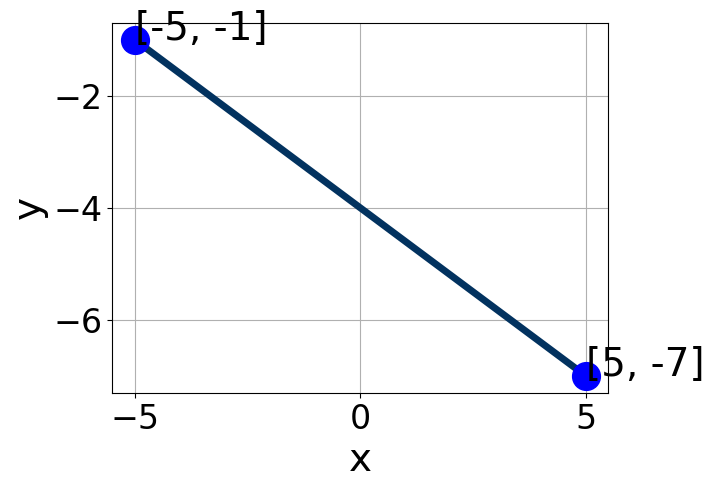
\includegraphics[width=0.5\textwidth]{../Figures/linearGraphToStandardCopyC.png}
\end{center}
\begin{enumerate}[label=\Alph*.]
\item \( A \in [2.1, 4.2], \hspace{3mm} B \in [4.1, 5.8], \text{ and } \hspace{3mm} C \in [-21, -14] \)
\item \( A \in [-3.8, -2.6], \hspace{3mm} B \in [-6.3, -3], \text{ and } \hspace{3mm} C \in [17, 25] \)
\item \( A \in [0.2, 1.2], \hspace{3mm} B \in [0.7, 3.9], \text{ and } \hspace{3mm} C \in [-7, -3] \)
\item \( A \in [0.2, 1.2], \hspace{3mm} B \in [-3.6, -0.1], \text{ and } \hspace{3mm} C \in [3, 6] \)
\item \( A \in [2.1, 4.2], \hspace{3mm} B \in [-6.3, -3], \text{ and } \hspace{3mm} C \in [17, 25] \)

\end{enumerate} }
\litem{
Solve the equation below. Then, choose the interval that contains the solution.\[ -17(8x + 6) = -15(-19x + 3) \]\begin{enumerate}[label=\Alph*.]
\item \( x \in [-0.43, -0.26] \)
\item \( x \in [0.19, 0.62] \)
\item \( x \in [-0.18, -0.07] \)
\item \( x \in [0.93, 1.06] \)
\item \( \text{There are no real solutions.} \)

\end{enumerate} }
\litem{
Solve the linear equation below. Then, choose the interval that contains the solution.\[ \frac{5x -6}{6} - \frac{8x -5}{7} = \frac{-7x -9}{8} \]\begin{enumerate}[label=\Alph*.]
\item \( x \in [0.98, 1.26] \)
\item \( x \in [-15.3, -14.1] \)
\item \( x \in [-1.6, -1.42] \)
\item \( x \in [-0.3, 0.43] \)
\item \( \text{There are no real solutions.} \)

\end{enumerate} }
\litem{
Write the equation of the line in the graph below in Standard form $Ax+By=C$. Then, choose the intervals that contain $A, B, \text{ and } C$.
\begin{center}
    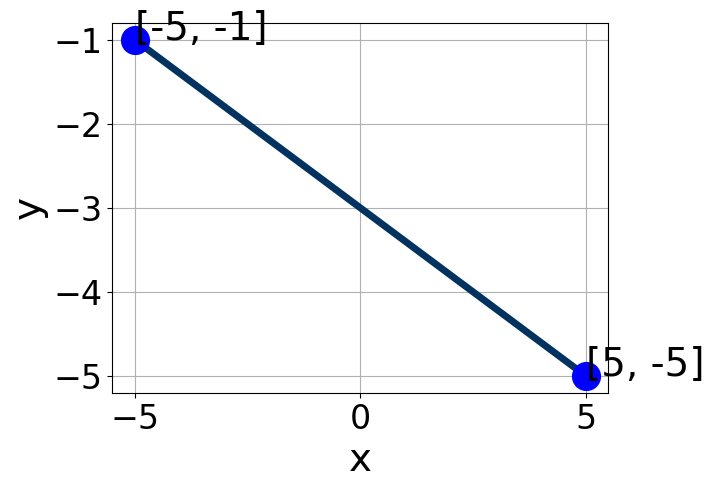
\includegraphics[width=0.5\textwidth]{../Figures/linearGraphToStandardC.png}
\end{center}
\begin{enumerate}[label=\Alph*.]
\item \( A \in [-0.84, 1.22], \hspace{3mm} B \in [-0.11, 1.52], \text{ and } \hspace{3mm} C \in [-6, 1] \)
\item \( A \in [1.72, 2.32], \hspace{3mm} B \in [4.04, 5.22], \text{ and } \hspace{3mm} C \in [-17, -9] \)
\item \( A \in [-3.8, -1.66], \hspace{3mm} B \in [-5.66, -4.56], \text{ and } \hspace{3mm} C \in [12, 20] \)
\item \( A \in [1.72, 2.32], \hspace{3mm} B \in [-5.66, -4.56], \text{ and } \hspace{3mm} C \in [12, 20] \)
\item \( A \in [-0.84, 1.22], \hspace{3mm} B \in [-1.39, -0.41], \text{ and } \hspace{3mm} C \in [3, 5] \)

\end{enumerate} }
\litem{
First, find the equation of the line containing the two points below. Then, write the equation as $ y=mx+b $ and choose the intervals that contain $m$ and $b$.\[ (-10, 5) \text{ and } (-6, -9) \]\begin{enumerate}[label=\Alph*.]
\item \( m \in [-3.5, 0.5] \hspace*{3mm} b \in [13.2, 16.6] \)
\item \( m \in [-3.5, 0.5] \hspace*{3mm} b \in [29.3, 31.4] \)
\item \( m \in [-3.5, 0.5] \hspace*{3mm} b \in [-33.1, -27] \)
\item \( m \in [0.5, 8.5] \hspace*{3mm} b \in [11, 13.7] \)
\item \( m \in [-3.5, 0.5] \hspace*{3mm} b \in [-3.6, -2] \)

\end{enumerate} }
\end{enumerate}

\end{document}